\section{Типы данных в языке С++: целый, вещественный,
символьный.}\label{ux442ux438ux43fux44b-ux434ux430ux43dux43dux44bux445-ux432-ux44fux437ux44bux43aux435-ux441-ux446ux435ux43bux44bux439-ux432ux435ux449ux435ux441ux442ux432ux435ux43dux43dux44bux439-ux441ux438ux43cux432ux43eux43bux44cux43dux44bux439.}

\textbf{Тип данных} - множество значений и операций над этими
значениями.

\begin{figure}
\centering
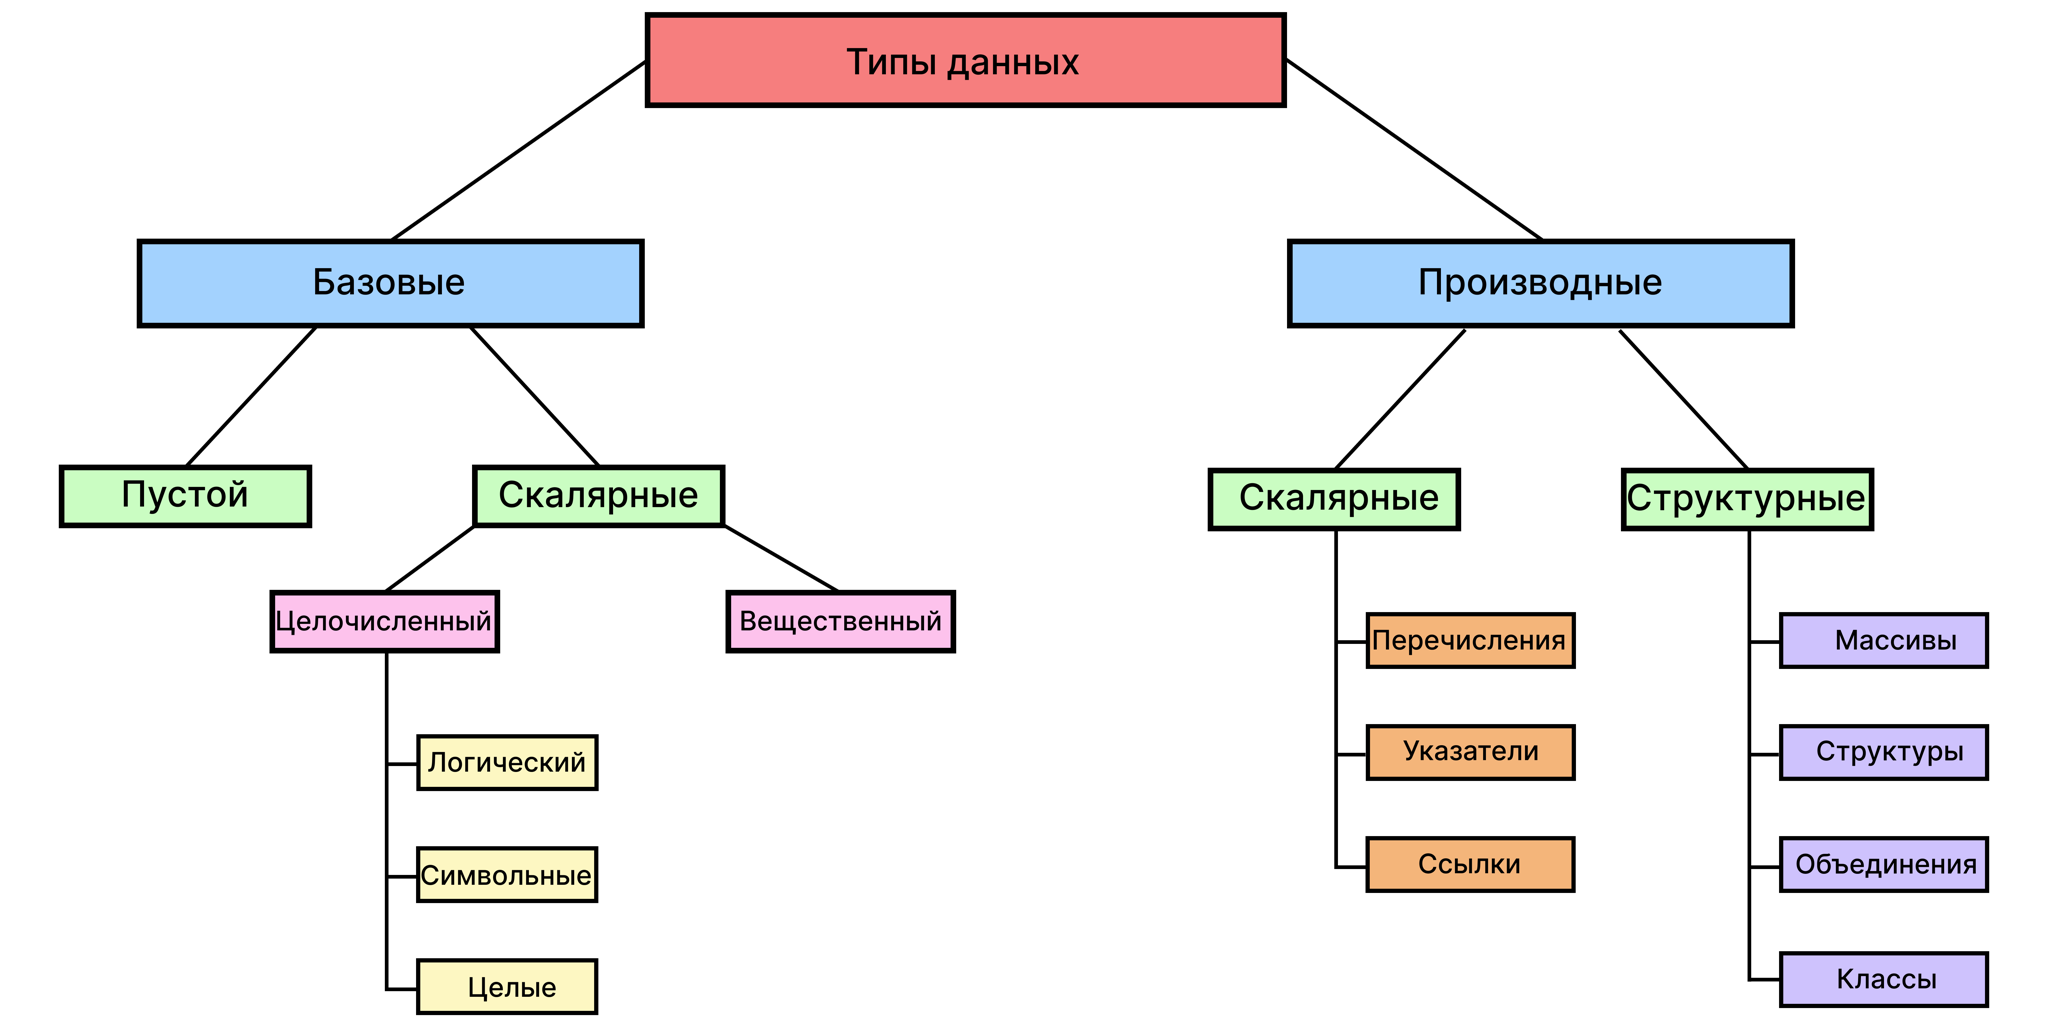
\includegraphics{./res/сpp-types.png}
\caption{Типы данных в C++}
\end{figure}

В категории базовых типов выделяют

\begin{enumerate}
\def\labelenumi{\arabic{enumi})}
\item
  Пустой тип (он же \texttt{void} в \textbf{С++}).

  Нет и не может быть объектов этого типа. Используется в отклонении
  (англ. \emph{discard}) результата вычисления (прим.
  \texttt{(void)GetAnswerToTheUniverse();}) и в функциях, не
  возвращающих значений.
\item
  Скалярные типы

  \begin{itemize}
  \tightlist
  \item
    Целочисленные типы: логический (\texttt{bool} в \textbf{С++}),
    символьный (\texttt{char}, \texttt{wchar\_t}, \texttt{char32\_t},
    \ldots), целый (\texttt{int}, \texttt{short}, \ldots)
  \item
    Вещественный тип
  \end{itemize}
\end{enumerate}

Отдельно рассмотрим целочисленные и вещественные типы данных в
\textbf{С++}.

\subsection{Целочисленные
типы}\label{ux446ux435ux43bux43eux447ux438ux441ux43bux435ux43dux43dux44bux435-ux442ux438ux43fux44b}

Стоит отметить, что размеры конкретных типов зависят от платформы.
Стандарт \textbf{С++} дает ограниченные гарантии на их размер. Также к
ключевым словам типов (\texttt{int}, \texttt{short}, \texttt{long})
могут добавляться квалификаторы \texttt{signed} (определяет знаковость)
и \texttt{unsigned} (определяет беззнаковость). Возможна и комбинация
ключевых слов типов: \texttt{unsigned\ long\ long\ int}.

\begin{longtable}[]{@{}
  >{\raggedright\arraybackslash}p{(\columnwidth - 12\tabcolsep) * \real{0.3418}}
  >{\raggedright\arraybackslash}p{(\columnwidth - 12\tabcolsep) * \real{0.1013}}
  >{\raggedright\arraybackslash}p{(\columnwidth - 12\tabcolsep) * \real{0.1139}}
  >{\raggedright\arraybackslash}p{(\columnwidth - 12\tabcolsep) * \real{0.0759}}
  >{\raggedright\arraybackslash}p{(\columnwidth - 12\tabcolsep) * \real{0.0844}}
  >{\raggedright\arraybackslash}p{(\columnwidth - 12\tabcolsep) * \real{0.1181}}
  >{\raggedright\arraybackslash}p{(\columnwidth - 12\tabcolsep) * \real{0.1646}}@{}}
\toprule\noalign{}
\begin{minipage}[b]{\linewidth}\raggedright
Тип
\end{minipage} & \begin{minipage}[b]{\linewidth}\raggedright
Эквивалентен
\end{minipage} & \begin{minipage}[b]{\linewidth}\raggedright
Пояснение
\end{minipage} & \begin{minipage}[b]{\linewidth}\raggedright
Минимальный размер
\end{minipage} & \begin{minipage}[b]{\linewidth}\raggedright
Размер на \emph{x86-64}
\end{minipage} & \begin{minipage}[b]{\linewidth}\raggedright
Диапазон значений (\emph{x86-64})
\end{minipage} & \begin{minipage}[b]{\linewidth}\raggedright
Примечание
\end{minipage} \\
\midrule\noalign{}
\endhead
\bottomrule\noalign{}
\endlastfoot
\texttt{signed\ char} & \texttt{signed\ char} & Символьный тип & 8 бит &
8 бит & -128 до 127 & \\
\texttt{unsigned\ char} & \texttt{unsigned\ char} & Символьный тип & 8
бит & 8 бит & 0 до 255 & \\
\texttt{char8\_t} & \texttt{char8\_t} & Символьный тип для UTF-8 & 8 бит
& 8 бит & 0 до 255 & С \textbf{С++20} \\
\texttt{wchar\_t} & \texttt{wchar\_t} & Длинный символьный тип & - &
зависит от платформы & зависит от платформы & На Unix/Linux - 32На
Windows - 16 \\
\texttt{char16\_t} & \texttt{char16\_t} & Символьный тип для UTF-16 & 16
бит & 16 бит & 0 до 65535 & \\
\texttt{char32\_t} & \texttt{char32\_t} & Символьный тип для UTF-32 & 32
бит & 32 бит & 0 до 1114111 (\emph{0x10ffff}) & Ограничение Unicode \\
\texttt{short}\texttt{short\ int}\texttt{signed\ short}\texttt{signed\ short\ int}
& \texttt{short\ int} & Целый тип, не больший \texttt{int} & 16 бит & 16
бит & −32768 до 32767 & \\
\texttt{unsigned\ short}\texttt{unsigned\ short\ int} &
\texttt{unsigned\ short\ int} & Беззнаковый \texttt{short} & 16 бит & 16
бит & 0 до 65535 & \\
\texttt{int}\texttt{signed}\texttt{signed\ int} & \texttt{int} &
Основной целый тип & 16 бит & 32 бит & \(-2^{31}\) до \(2^{31}-1\) & \\
\texttt{unsigned}\texttt{unsigned\ int} & \texttt{unsigned\ int} &
Беззнаковый \texttt{int} & 16 бит & 32 бит & 0 до \(2^{32}-1\) & \\
\texttt{long}\texttt{long\ int}\texttt{signed\ long}\texttt{signed\ long\ int}
& \texttt{long\ int} & \emph{Длинное} целое & 32 бит & зависит от
платформы & зависит от платформы & На Unix/Linux - 64Windows API - 32 \\
\texttt{unsigned\ long}\texttt{unsigned\ long\ int} &
\texttt{unsigned\ long\ int} & Беззнаковый \texttt{long} & 32 бит &
зависит от платформы & зависит от платформы & На Unix/Linux - 64Windows
API - 32 \\
\texttt{long\ long}\texttt{long\ long\ int}\texttt{signed\ long\ long}\texttt{signed\ long\ long\ int}
& \texttt{long\ long\ int} & \emph{Дважды длинное} целое & 64 бит & 64
бит & \(-2^{63}\) до \(2^{63}-1\) & \\
\texttt{unsigned\ long\ long}\texttt{unsigned\ long\ long\ int} &
\texttt{unsigned\ long\ long\ int} & Беззнаковый \texttt{long\ long} &
64 бит & 64 бит & 0 до \(2^{64}-1\) & \\
\end{longtable}

\begin{quote}
Тип \texttt{char} занимает по крайней мере 8 бит и ведет себя так же,
как и \texttt{signed\ char} или \texttt{unsigned\ char}, но является
отдельным типом. При этом конкретная знаковость зависит от платформы и
настроек компилятора. На \emph{x86} он обычно знаковый, на \emph{arm} -
обычно беззнаковый.
\end{quote}

\begin{quote}
Логический тип \texttt{bool} занимает по крайней мере 8 бит и хранит
лишь два значения - \texttt{true} или \texttt{false}.
\end{quote}

Типы в \textbf{С++} формируют иерархию по размеру:

\begin{Shaded}
\begin{Highlighting}[]
    \DecValTok{1} \OperatorTok{==} \KeywordTok{sizeof}\OperatorTok{(}\DataTypeTok{char}\OperatorTok{)}\NormalTok{ ≤ }\KeywordTok{sizeof}\OperatorTok{(}\DataTypeTok{short}\OperatorTok{)}\NormalTok{ ≤ }\KeywordTok{sizeof}\OperatorTok{(}\DataTypeTok{int}\OperatorTok{)}\NormalTok{ ≤ }\KeywordTok{sizeof}\OperatorTok{(}\DataTypeTok{long}\OperatorTok{)}\NormalTok{ ≤ }\KeywordTok{sizeof}\OperatorTok{(}\DataTypeTok{long} \DataTypeTok{long}\OperatorTok{)}
\end{Highlighting}
\end{Shaded}

Однако стандарт гарантирует лишь минимальное количество бит типов. В
частности возможная абсурдная ситуация, когда на платформе один байт*
занимает 64 бит и

\begin{Shaded}
\begin{Highlighting}[]
    \KeywordTok{sizeof}\OperatorTok{(}\DataTypeTok{char}\OperatorTok{)} \OperatorTok{==} \KeywordTok{sizeof}\OperatorTok{(}\DataTypeTok{short}\OperatorTok{)} \OperatorTok{==} \KeywordTok{sizeof}\OperatorTok{(}\DataTypeTok{int}\OperatorTok{)} \OperatorTok{==} \KeywordTok{sizeof}\OperatorTok{(}\DataTypeTok{long}\OperatorTok{)} \OperatorTok{==} \KeywordTok{sizeof}\OperatorTok{(}\DataTypeTok{long} \DataTypeTok{long}\OperatorTok{)} \OperatorTok{==} \DecValTok{1}
\end{Highlighting}
\end{Shaded}

Количество бит, которое занимает тип \texttt{char} можно проверить
макросом \texttt{CHAR\_BIT}; впрочем, практически все современные
системы имеют байт* равным 8 бит.

*под байтом в этом контексте понимается минимально адресуемый объем
памяти. Это не обязательно `байт' в значении объем информации.

\subsection{Вещественные
типы}\label{ux432ux435ux449ux435ux441ux442ux432ux435ux43dux43dux44bux435-ux442ux438ux43fux44b}

Стандарт \textbf{С++} определяет следующие типы с плавающей точкой: 1)
\texttt{float} - вещественный тип одинарной точности. Обычно
\textbf{IEEE 754} \emph{binary32}. 2) \texttt{double} - вещественный тип
двойной точности. Обычно \textbf{IEEE 754} \emph{binary64}. 3)
\texttt{long\ double} - вещественный тип повышенной точности.

\begin{verbatim}
На разных платформах может быть типом четверной точности (**IEEE 754** *binary128*), 80-битным *x87-80 extended precision format* на *x86*, быть эквивалентным `double` или реализован каким-либо другим образом.
\end{verbatim}
